\documentclass[a4paper,12pt]{article}

\usepackage{geometry}
\geometry{margin=1in}

\usepackage{enumitem}
\usepackage{graphicx}
\usepackage{float}
\usepackage{tikz}
\usetikzlibrary{shapes,arrows}
\usepackage{caption}

\begin{document}
	
	\title{RS485 Wired Network Specification}
	\author{Michael King}
	\date{\today}
	
	\maketitle
	
	\section{Introduction}
	
	This document provides a detailed specification for the RS485-based wired network. It outlines the components, protocols, and configurations necessary for the successful implementation and operation of the network.
	
	\section{Network Topology}
	
	Physical layout and topology:
	
	\subsection{Wireless topology}
	The wireless network will be an xbee mesh using zigbee modules.
	
	\subsection{Wired network}
	The wired network is based on the RS485 physical standard.
	The wired network will use a bus topology, with all devices connected in series and terminated using 120$\Omega$ resistors.
	
	\section{Hardware Components}
	
	List and describe the hardware components involved in the network:
	\subsection{wireless}
	The wireless network is based on our xbee modules.
	\subsection{wired}
	The wired network is based on the RS485 standard, with our own handling for messages.
	\subsubsection{Network devices}
	The network consists of one Master device, with up to 255 subordinate devices in a single bus.
	\subsubsection{RS485 transceiver}
	The selected transceiver allows for up to 16mbps communication, and up to 255 receiving devices on a network.
	(include a reference link to the RS485 transceiver)
	\subsubsection{power supply}
	The master device is capable of supplying up to 11w on each port.
	
	\subsubsection{Cables and connectors}
	The expected connector is a generic RJ45.
	With cables ranging from cat5e to cat6.
	A single twisted pair is for data transmission, the other three are for power.
	
	\subsubsection{Termination resistors}
	The bus should be terminated with a 120$\Omega$ resistance on each end.
	
	\section{Communication Protocol}
	
	\subsection{Wireless}
	the wireless network is dependent on the built in protocols of the xbee modules.
	
	\subsection{Wired}
	Detail the communication protocol used on the RS485 network. Include information on:
	
	\subsubsection{Baud rate}
	
	we are expecting a bit rate of around 115200.
	
	\section{Data Frames}
	
	Describe the format of data frames used in the RS485 network. Include details such as:
	
	\begin{itemize}[label=--]
		\item Start and stop bits.
		\item Data length.
		\item Addressing scheme.
		\item Payload structure.
	\end{itemize}
	
	     \begin{figure}[htp]
		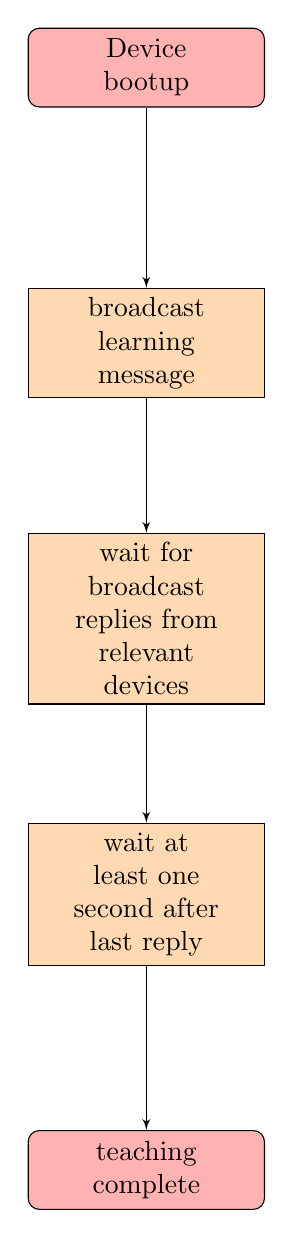
\begin{tikzpicture}[auto, node distance=3cm,>=latex']
			%define block styles
			\tikzset{
				startstop/.style={rectangle, rounded corners, minimum width=3cm, text width=6em, minimum height=1cm, text centered, draw=black, fill=red!30},
				process/.style={rectangle, minimum width=3cm, minimum height=1cm, text width=6em, text centered, draw=black, fill=orange!30},
				decision/.style={diamond, minimum width=3cm, minimum height=1cm, text width=6em, text centered, draw=black, fill=green!30},
				arrow/.style={thick,->,>=stealth},
			}
			%define nodes
			\node[startstop](boot){Device bootup};
			\node[process, below of=boot, yshift=-0.5cm](teach){broadcast learning message};
			\node[process, below of=teach, yshift=-0.5cm](wait){wait for broadcast replies from relevant devices};
			\node[process, below of=wait, yshift=-0.5cm](loop){wait at least one second after last reply};
			\node[startstop, below of=loop, yshift=-0.5cm](done){teaching complete};
			%define arrows
			\draw[->] (boot) -- (teach);
			\draw[->] (teach) -- (wait);
			\draw[->] (wait) -- (loop);
			\draw[->] (loop) -- (done);
		\end{tikzpicture}
		\caption{Wireless device teach routine high-level flowchart}\label{fig:simpleflowteach}
	\end{figure}
	\begin{figure}[htp]
		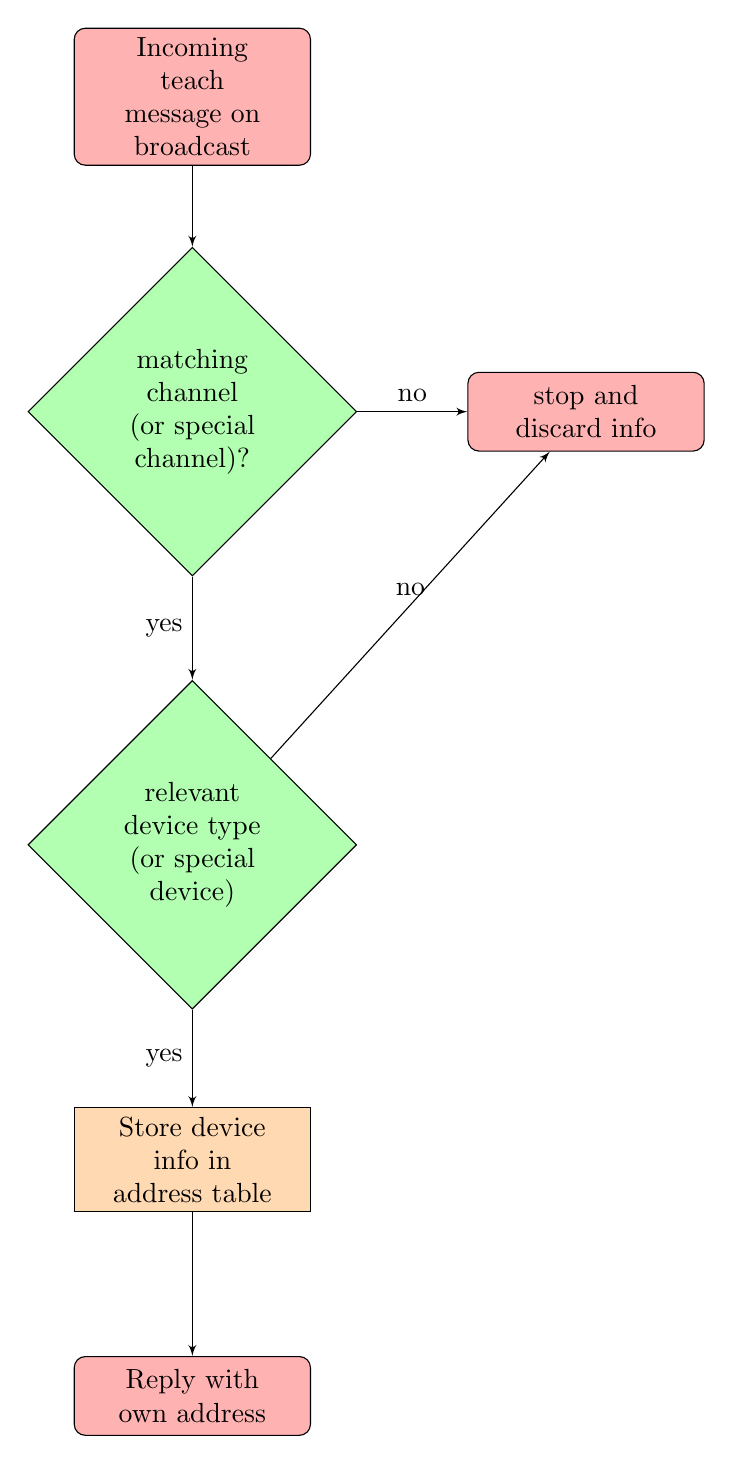
\begin{tikzpicture}[auto, node distance=3cm,>=latex']
			\tikzset{
				startstop/.style={rectangle, rounded corners, minimum width=3cm, text width=6em, minimum height=1cm, text centered, draw=black, fill=red!30},
				process/.style={rectangle, minimum width=3cm, minimum height=1cm, text width=6em, text centered, draw=black, fill=orange!30},
				decision/.style={diamond, minimum width=3cm, minimum height=1cm, text width=6em, text centered, draw=black, fill=green!30},
				arrow/.style={thick,->,>=stealth},
			}
			\node[startstop](learn){Incoming teach message on broadcast};
			\node[decision, below of=learn, yshift=-1cm](channel){matching channel (or special channel)?};
			\node[startstop, right of=channel, xshift=2cm](discard){stop and discard info};
			\node[decision, below of=channel, yshift=-2.5cm](device){relevant device type (or special device)};
			\node[process, below of=device, yshift=-1cm](store){Store device info in address table};
			\node[startstop, below of=store](reply){Reply with own address};
			%draw arrows
			\draw[->] (learn) -- (channel);
			\draw[->] (channel) -- node[above] {no} (discard);
			\draw[->] (channel) -- node[anchor=east] {yes} (device);
			\draw[->] (device) -- node[anchor=east] {yes} (store);
			\draw[->] (device) -- node[above] {no} (discard);
			\draw[->] (store) -- (reply);
		\end{tikzpicture}
		\caption{Device learn flowchart for the wireless and wired network}
		\label{fig:simpleflowlearn}
	\end{figure}
	\begin{figure}[htp]
		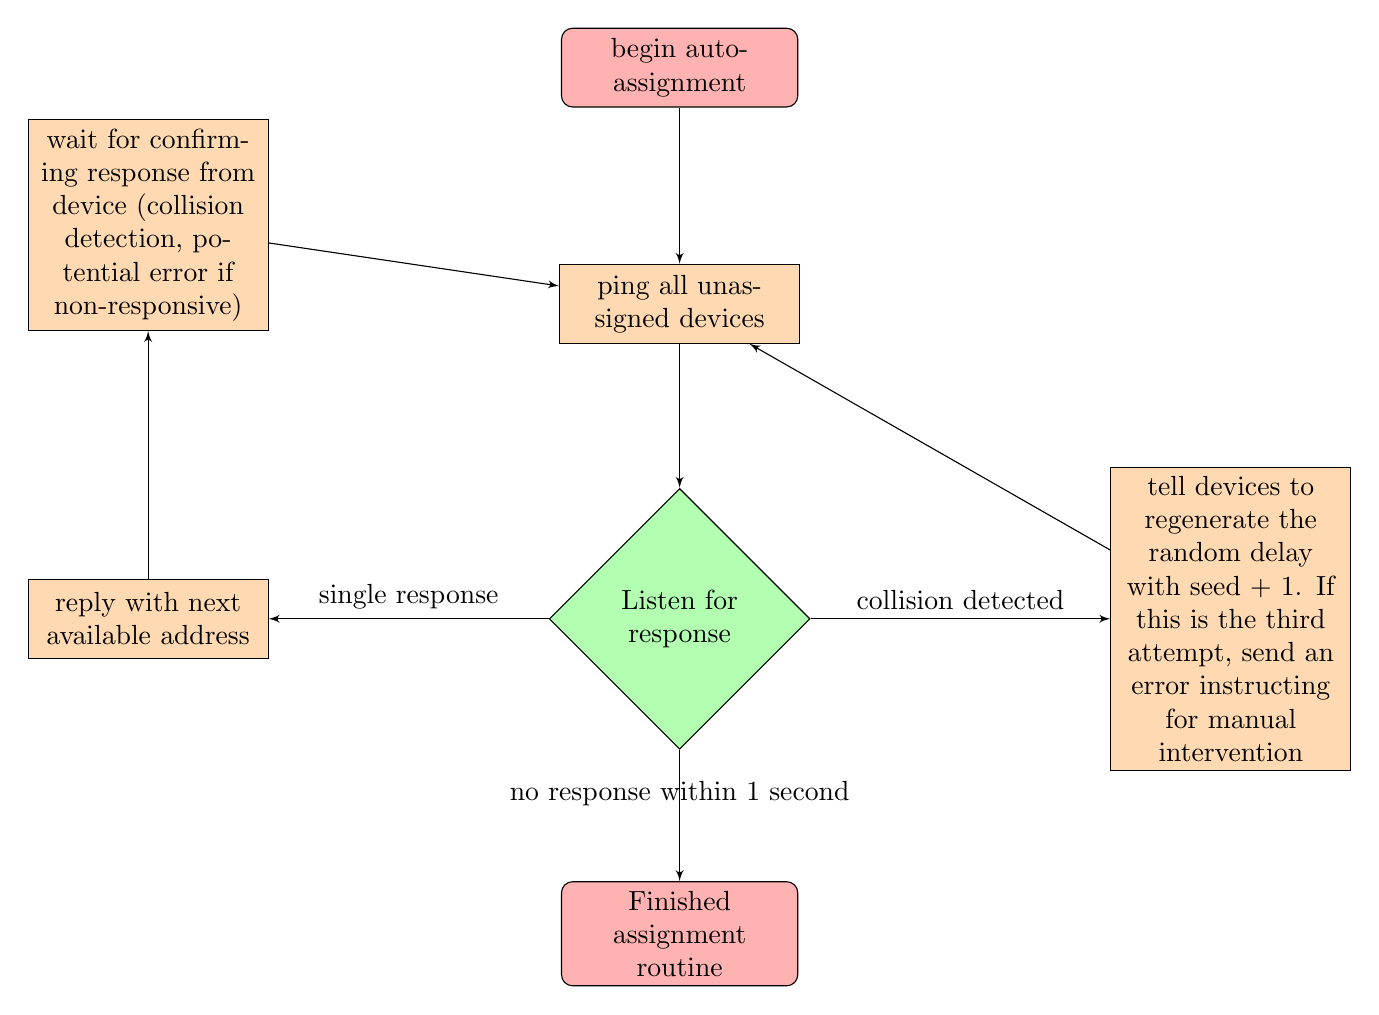
\begin{tikzpicture}[auto, node distance=3cm,>=latex']
			\tikzset{
				startstop/.style={rectangle, rounded corners, minimum width=3cm, text width=6em, minimum height=1cm, text centered, draw=black, fill=red!30},
				process/.style={rectangle, minimum width=3cm, minimum height=1cm, text width=8em, text centered, draw=black, fill=orange!30},
				decision/.style={diamond, minimum width=3cm, minimum height=1cm, text width=6em, text centered, draw=black, fill=green!30},
				arrow/.style={thick,->,>=stealth},
			}
			\node[startstop](start){begin auto-assignment};
			\node[process, below of=start](ping){ping all unassigned devices};
			\node[decision, below of=ping, yshift=-1cm](listen){Listen for response};
			\node[startstop, below of=listen, yshift=-1cm](done){Finished assignment routine};
			\node[process, left of=listen, xshift=-3.75cm](assign){reply with next available address};
			\node[process, above of=assign, yshift=2cm](confirm){wait for confirming response from device (collision detection, potential error if non-responsive)};
			\node[process, right of=listen, xshift=4cm](collide){tell devices to regenerate the random delay with seed + 1. If this is the third attempt, send an error instructing for manual intervention};
			%draw arrows
			\draw[->] (start) -- (ping);
			\draw[->] (ping) -- (listen);
			\draw[->] (listen) -- node[above] {single response} (assign);
			\draw[->] (assign) -- (confirm);
			\draw[->] (confirm) -- (ping);
			\draw[->] (collide) -- (ping);
			\draw[->] (listen) -- node[above] {no response within 1 second} (done);
			\draw[->] (listen) -- node[above] {collision detected} (collide);
		\end{tikzpicture}
		\caption{Auto-assign routine flow chart for the wired network}
		\label{fig:autoassignflow}
	\end{figure}
	\begin{figure}
		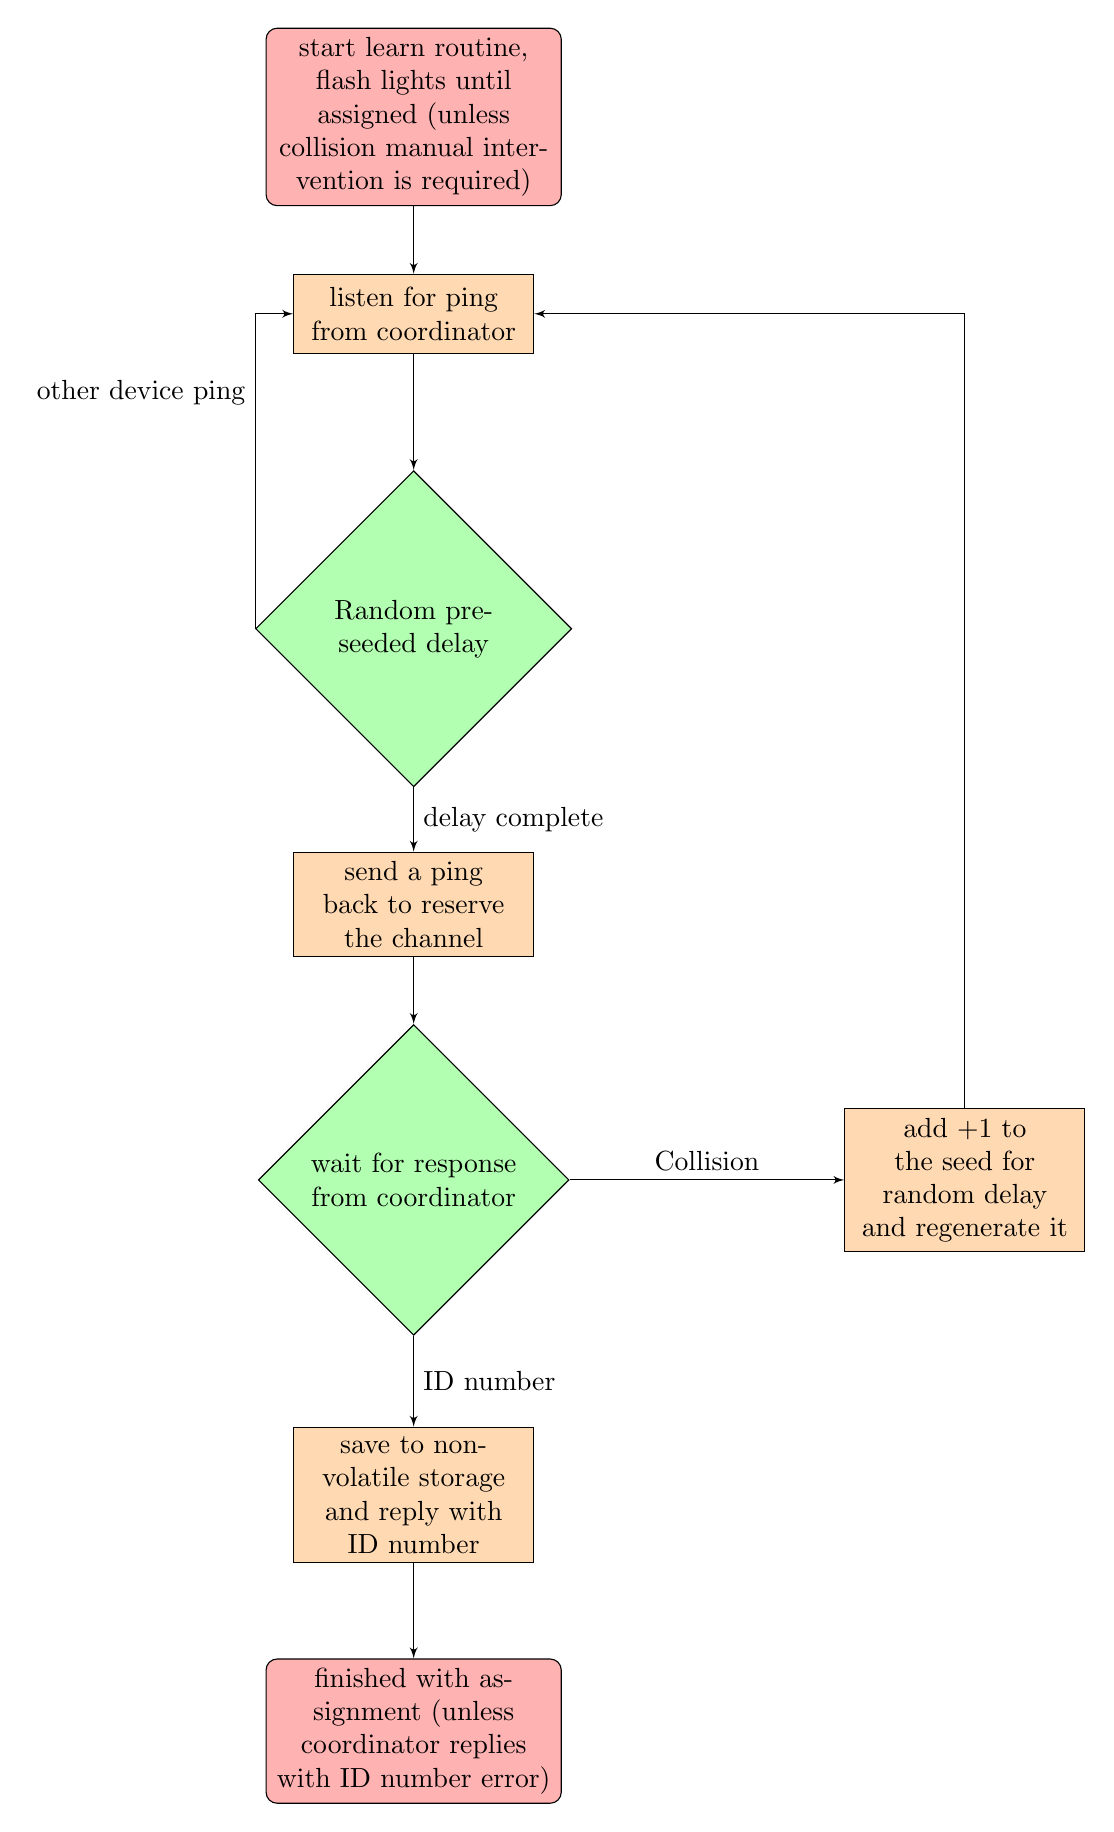
\begin{tikzpicture}[auto, node distance=3cm,>=latex']
			\tikzset{
				startstop/.style={rectangle, rounded corners, minimum width=3cm, text width=10em, minimum height=1cm, text centered, draw=black, fill=red!30},
				process/.style={rectangle, minimum width=3cm, minimum height=1cm, text width=8em, text centered, draw=black, fill=orange!30},
				decision/.style={diamond, minimum width=3cm, minimum height=1cm, text width=8em, text centered, draw=black, fill=green!30},
				arrow/.style={thick,->,>=stealth},
			}
			\node[startstop](start){start learn routine, flash lights until assigned (unless collision manual intervention is required)};
			\node[process, below of=start, yshift=0.5cm](listen){listen for ping from coordinator};
			\node[decision, below of=listen, yshift=-1cm](delay){Random pre-seeded delay};
			\node[process, below of=delay, yshift=-0.5cm](pingback){send a ping back to reserve the channel};
			\node[decision, below of=pingback, yshift=-0.5cm](listen2){wait for response from coordinator};
			\node[process, right of=listen2, xshift=4cm](collision){add +1 to the seed for random delay and regenerate it};
			\node[process, below of=listen2, yshift=-1cm](learn){save to non-volatile storage and reply with ID number};
			\node[startstop,below of=learn](finished){finished with assignment (unless coordinator replies with ID number error)};
			%Draw arrows
			\draw[->] (start) -- (listen);
			\draw[->] (listen) -- (delay);
			\draw[->] (delay) -- node[right] {delay complete} (pingback);
			\draw[->] (delay.west) |- node[left, yshift=-1cm] {other device ping} (listen);
			\draw[->] (pingback) -- (listen2);
			\draw[->] (listen2) -- node[above] {Collision} (collision);
			\draw[->] (collision) |- (listen);
			\draw[->] (listen2) -- node[right] {ID number} (learn);
			\draw[->] (learn) -- (finished);
		\end{tikzpicture}
		\caption{auto-learn routine on the wired network}
		\label{fig:autolearnwiredflow}
	\end{figure}
	\section{Conclusion}
	
	Summarize the key points of the RS485 wired network specification and emphasize any critical considerations for successful implementation.
	
\end{document}
